\documentclass[11pt, floatsintext]{apa6}
\usepackage{amssymb}
\usepackage{graphicx}
\usepackage[outdir=./]{epstopdf}
%\DeclareGraphicsExtensions{.eps}

\usepackage{mathtools}
\usepackage{enumerate}
\usepackage{apacite}
\usepackage{listings}
\usepackage{multirow}
\usepackage{todonotes}
\usepackage{svg}
\usepackage{booktabs}


\newcommand{\den}[2][]{
\(
\left\llbracket\;\text{#2}\;\right\rrbracket^{#1}
\)
}

\synctex=1
\usepackage{soul}

\newcommand{\KL}[2]{\ensuremath{D_{KL}({#1}\, \| \, {#2})}}
\newcommand{\E}[2]{\ensuremath{\mathbb{E}_{#1}\left [#2 \right]}}

\newenvironment{figurehere}
	{\def\@captype{figure}}
	{}

\usepackage{lipsum}
%\pagenumbering{gobble}
%\usepackage{apacite}

\linespread{1}
\usepackage{textcomp}
\usepackage{lingmacros}

\DeclareGraphicsRule{.tif}{png}{.png}{`convert #1 `dirname #1`/`basename #1 .tif`.png}
\graphicspath{{./figures/}}
 
 \definecolor{Green}{RGB}{10,200,100}
  \definecolor{Red}{RGB}{200,100,50}
\newcommand{\ndg}[1]{\textcolor{Green}{[ndg: #1]}}  
\newcommand{\rdh}[1]{\textcolor{Red}{[rdh: #1]}}  


\makeatother

\title{An inferential theory of convention formation}
\shorttitle{Conventions}
\author{Authors}
\affiliation{Universities}

\abstract{Abstract}


\keywords{keywords}

\authornote{This report is based in part on work presented at the 38th Conference of the Cognitive Science Society. Correspondence should be addressed to Robert D. Hawkins, e-mail: rdhawkins@princeton.edu}

\begin{document}
\maketitle

%\section{Introduction}
%
%\subsection{Cognitive theories of local alignment}
%
%Interactive alignment theories say that coordination is `priming' with some connectionist voodoo that trickles up levels. 
%
%\subsection{Distributed network theories of global convergence}
%
%Agent-based models use heuristics 
%
%\section{Convention formation as hierarchical inference}
%
%We present our model. It is learning and inference all the way down but gives rise to emergent behavior in groups.
%
%\section{Experiment 1: pragmatic inferences shape conventions}
%
%We run some simulations and fit our model to an artificial language communication game. 
%
%We make the point that our model (by virtue of bayesian inference machinery) explains the way context shapes conventions in ways that other models cannot.
%
%\subsection{Simulations}
%
%We show conditions under which you see convergence. 
%
%\subsection{Experimental design}
%
\section{Experiment 2: generalization to new partners in a social network}

How do \emph{ad hoc} conventions formed through interaction with a single partner become \emph{global} conventions shared throughout a community?
In this section, we provide an explicit computational account of the cognitive mechanisms driving this shift.
The key predictions distinguishing our model concern the pattern of generalization across partners.
First, we show that our model accounts for the \emph{partner-specificity} of ad hoc conventions as a consequence of hierarchical structure. 
Under our model, speakers revert back to a longer description with a novel partner because evidence from a single listener is relatively uninformative about the community-level prior.

This hierarchical structure, however, leads to a further prediction: after interacting with enough partners in a tight-knit community, speakers should become increasingly confident that labels are not simply idiosyncratic features of a particular partner's lexicon but are shared across the entire community.
In other words, the partner-specific expectations agents form within an interaction to solve a novel communication problem should gradually generalize to community-wide expectations as they gain additional evidence of the latent population-level distribution from which different partners are sampled.
These expectations should manifest in an increasing willingness to use short labels with novel partners, leading to the emergent consequence of lending additional evidence for that structure. 
We test this novel prediction in a networked communication game and compare our model to two non-hierarchical variants: a `complete-pooling' model that collapses across partners and a `no-pooling' model that treats partners as entirely separate.

\begin{figure}[t!]
\centering
    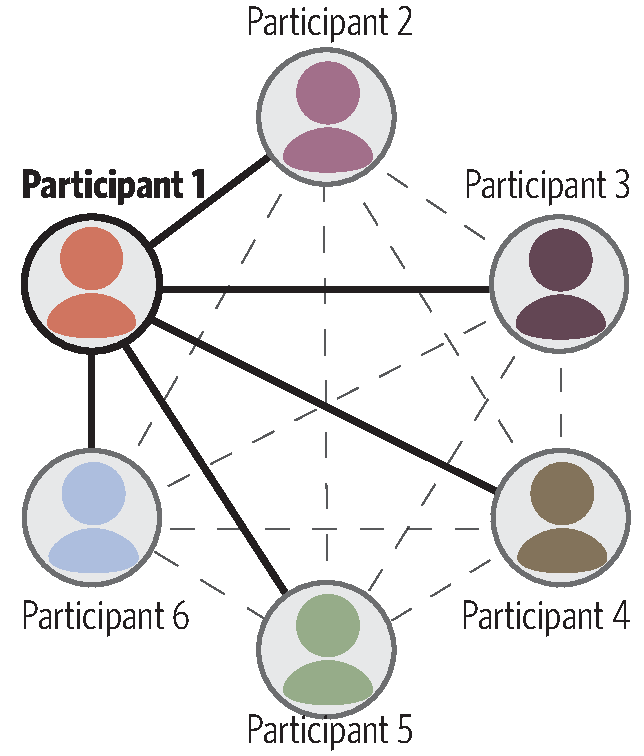
\includegraphics[scale=.32]{task1_network.pdf}
  \caption{Network}% tying individual cognition to population-level patterns}
  \label{fig:task1_network}
\end{figure}

\subsection{Participants}

We recruited 600 participants from Amazon Mechanical Turk to play an interactive, natural-language reference game using the Dallinger platform\footnote{http://docs.dallinger.io/}.
Participants were randomly assigned to one of 100 six-member networks and embedded as a fully-connected graph, such that everyone was neighbors with everyone else in their assigned community (Fig. \ref{fig:task1_network}). 
We prescreened participants who report a native language different from English. 

\subsection{Stimulus \& design}

%At a high level, my experiment design will follow the basic setup from \cite{fay_interactive_2010}. 
Participants were paired with each of their five neighbors in a round-robin schedule.
In each interaction, they played a game where they repeatedly referred to six abstract tangram shapes taken from \citeA[Fig. \ref{fig:task1_display}]{clark_referring_1986}.
These stimuli have been used extensively in the literature on coordination and common ground \shortcite<e.g.>{duff_development_2006,hawkins_convention-formation_2017}.
They were designed such that participants will not already have strong pre-existing lexical conventions for how to refer to them (unlike photographs of common objects), but are structured enough to support many possible descriptions (unlike images of white noise).

On each trial of a reference game, one of these six shapes was highlighted as the \emph{target object} for the ``speaker'' who was instructed to use a chatbox to communicate the identity of this object to their partner, the ``listener''.
The listener may reply through the chatbox but must ultimately make a selection from the array. 
The trial sequence for a given partner was constructed so that each of four targets appear six times each, spread evenly across the session, for a total of 24 trials.

After completing 24 trials with one partner, they were introduced to their next partner and asked to play the repeated reference game again with the same four objects.
Each participant in a network was assigned a distinct avatar so that participants were clear they were speaking to distinct partners.
This process repeated until each participant had partnered with all five neighbors.
Players were given full feedback on each about their partner's choice and received bonus payment for each correct response. 
Because some pairs within the network took longer than others to complete the trial sequence, we sent participants to a temporary waiting room if their next partner was not yet ready. 

\todo[inline]{A remaining design decision is how to handle disconnections in the middle of the game. do we immediately terminate the entire group as soon as one person drops out? Do we just continue the game without them, making whoever was supposed to be their partner wait a long time? do we recruit to fill their place? my first thought is to just terminate the group to minimize turker frustration (i.e. more will probably dropout if they have to wait because of the first dropout) and to avoid having to account for newly recruited turkers in the analysis}

\begin{figure}
\centering
    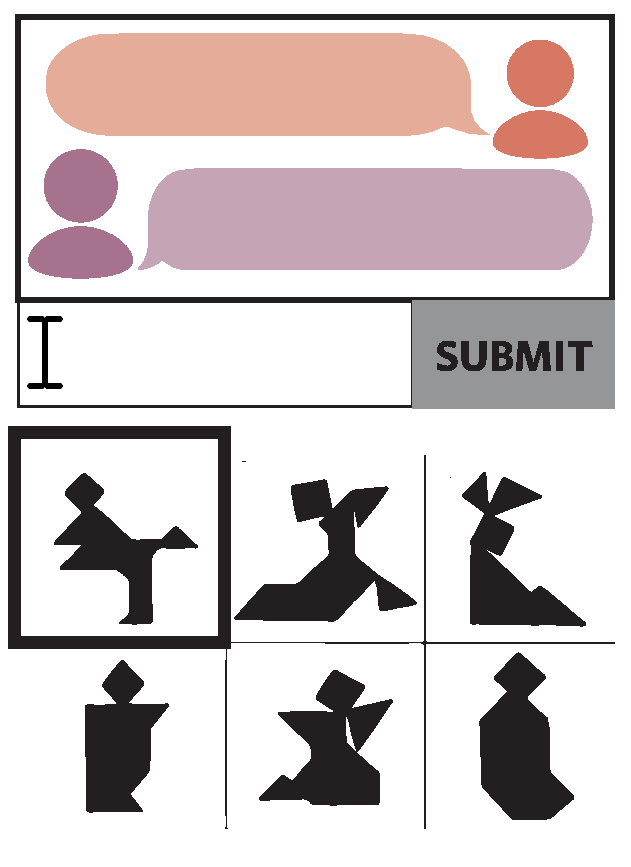
\includegraphics[scale=.27]{task1_display.pdf}
  \caption{Task}% tying individual cognition to population-level patterns}
  \label{fig:task1_display}
\end{figure}


\subsection{Confirmatory behavioral predictions}
%A partial pooling account makes three behavioral predictions that allow us to distinguish it from no pooling and complete pooling accounts. 
The most diagnostic dependent variable to distinguish the hierarchical model from alternatives concerns the mean number of words used per description.
This is a common operationalization of conventionalization in terms of coding efficiency.
In particular, we are interested in how this measure changes within partners and across partner boundaries.
The first panel of Fig. \ref{fig:task1predictions} shows the mean number of words used across six repetitions with one partner in a pilot experiment with $N=100$ isolated pairs.
All of the model variants we consider are consistent with this pattern: messages reduce in length across repetitions with a partner as they coordinate on shorthand. 

However, our account diverges in its predictions at the partner boundary, as visualized in the remaining panels of Fig. \ref{fig:task1predictions}. 
Pilot data was used to calibrate expected effect sizes. 
While `complete-pooling' predicts that participants will completely transfer conventions from the previous partner  \cite<inconsistent with existing evidence from psycholinguistics, e.g.>{wilkes-gibbs_coordinating_1992}, the other accounts predict that speakers will revert nearly to their initial description length.
Furthermore, while \emph{no-pooling} predicts the same complete reversion with every subsequent partner, our hierarchical \emph{partial pooling} account predicts that the magnitude of the reversion will decrease over successive interactions: after several partners, it predicts transfer as strongly as complete pooling. 

\begin{figure}
\centering
    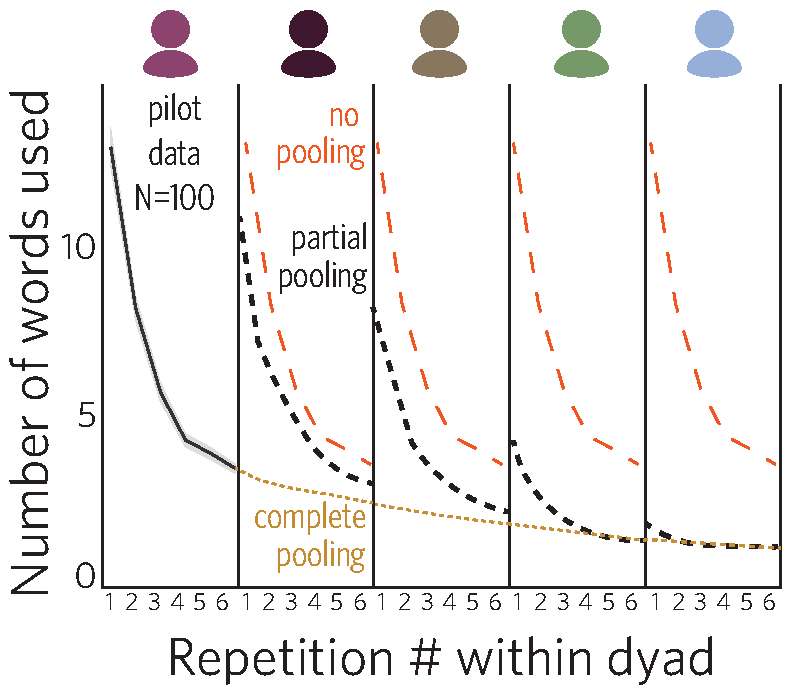
\includegraphics[scale=.5]{task1_predictions.pdf}
  \caption{Predictions}% tying individual cognition to population-level patterns}
  \label{fig:task1predictions}
\end{figure}

We will test these predictions using a mixed-effects regression of partner number on ``reversion size'' (the difference in number of words between the final descriptions on one repetition and the initial ones on the next), with maximum random-effect structure including item-effects at the object and speaker level.  
Only the partial pooling model predicts a significant decrease in reversion over successive partners. 
Preliminary support for this signature was reported by \shortciteA{fay_interactive_2010} in a Pictionary task where participants used sketches to communicate verbal concepts instead of using words to refer to visual targets, and the measure of interest was the  complexity of the drawings \cite<see also>{garrod_conversation_1994}.

\subsection{Simulations}

\section{\bf Acknowledgments}
\small

\bibliography{ref}
\bibliographystyle{apacite}


\end{document}  
